\documentclass{article}
\usepackage[utf8]{inputenc}

\usepackage{amssymb,amsmath,amsthm}
\usepackage{mathtools}

% Links, references
\usepackage{url}            % simple URL typesetting
\usepackage[colorlinks=true]{hyperref}

\newtheorem{theorem}{Theorem}[section]
\newtheorem{corollary}{Corollary}[section]
\newtheorem{lemma}{Lemma}[section]
\newtheorem{proposition}{Proposition}[section]

\theoremstyle{definition}
\newtheorem{definition}{Definition}[section]
\newtheorem{remark}{Remark}[section]
\newtheorem{example}{Example}[section]
\newtheorem{question}{Question}[section]
%Elementary functions
\newcommand{\floor}[1]{\left\lfloor #1 \right\rfloor}
\newcommand{\ceil}[1]{\left\lceil #1 \right\rceil}
\newcommand{\abs}[1]{\left\lvert #1 \right\rvert}
\newcommand{\by}{\times}
 
%Vector/matrix calculus
\newcommand{\norm}[1]{\left\lVert #1 \right\rVert}
\newcommand{\ip}[1]{\left\langle #1 \right\rangle}
\newcommand{\grad}{\nabla}

%Sets
\let\oldemptyset\emptyset
\let\emptyset\varnothing
\newcommand{\set}[1]{\left\{#1\right\}}

%Letters in different typefaces
%\newcommand{\A}{\mathbb{A}}
\def\A{{\mathbb{A}}}
\def\B{{\mathbb{B}}}
\def\C{{\mathbb{C}}}
\def\D{{\mathbb{D}}}
% \def\E{{\mathbb{E}}}
\def\F{{\mathbb{F}}}
\def\G{{\mathbb{G}}}
\def\H{{\mathbb{H}}}
\def\I{{\mathbb{I}}}
\def\J{{\mathbb{J}}}
\def\K{{\mathbb{K}}}
\def\L{{\mathbb{L}}}
\def\M{{\mathbb{M}}}
\def\N{{\mathbb{N}}}
\def\O{{\mathbb{O}}}
\def\P{{\mathbb{P}}}
\def\Q{{\mathbb{Q}}}
\def\R{{\mathbb{R}}}
\def\S{{\mathbb{S}}}
\def\T{{\mathbb{T}}}
\def\U{{\mathbb{U}}}
\def\V{{\mathbb{V}}}
\def\W{{\mathbb{W}}}
\def\X{{\mathbb{X}}}
\def\Y{{\mathbb{Y}}}
\def\Z{{\mathbb{Z}}}

\def\bA{{\mathbf{A}}}
\def\bB{{\mathbf{B}}}
\def\bC{{\mathbf{C}}}
\def\bD{{\mathbf{D}}}
\def\bE{{\mathbf{E}}}
\def\bF{{\mathbf{F}}}
\def\bG{{\mathbf{G}}}
\def\bH{{\mathbf{H}}}
\def\bI{{\mathbf{I}}}
\def\bJ{{\mathbf{J}}}
\def\bK{{\mathbf{K}}}
\def\bL{{\mathbf{L}}}
\def\bM{{\mathbf{M}}}
\def\bN{{\mathbf{N}}}
\def\bO{{\mathbf{O}}}
\def\bP{{\mathbf{P}}}
\def\bQ{{\mathbf{Q}}}
\def\bR{{\mathbf{R}}}
\def\bS{{\mathbf{S}}}
\def\bT{{\mathbf{T}}}
\def\bU{{\mathbf{U}}}
\def\bV{{\mathbf{V}}}
\def\bW{{\mathbf{W}}}
\def\bX{{\mathbf{X}}}
\def\bY{{\mathbf{Y}}}
\def\bZ{{\mathbf{Z}}}

\def\cA{{\mathcal A}}
\def\cB{{\mathcal B}}
\def\cC{{\mathcal C}}
\def\cD{{\mathcal D}}
\def\cE{{\mathcal E}}
\def\cF{{\mathcal F}}
\def\cG{{\mathcal G}}
\def\cH{{\mathcal H}}
\def\cI{{\mathcal I}}
\def\cJ{{\mathcal J}}
\def\cK{{\mathcal K}}
\def\cL{{\mathcal L}}
\def\cM{{\mathcal M}}
\def\cN{{\mathcal N}}
\def\cO{{\mathcal O}}
\def\cP{{\mathcal P}}
\def\cQ{{\mathcal Q}}
\def\cR{{\mathcal R}}
\def\cS{{\mathcal S}}
\def\cT{{\mathcal T}}
\def\cU{{\mathcal U}}
\def\cV{{\mathcal V}}
\def\cW{{\mathcal W}}
\def\cX{{\mathcal X}}
\def\cY{{\mathcal Y}}
\def\cZ{{\mathcal Z}}

%Optimization basics
\newcommand{\Opt}{\operatorname{Opt}}
\newcommand{\argmin}{\operatorname*{arg\,min}}
\newcommand{\argmax}{\operatorname*{arg\,max}}

%Matrix related
\newcommand{\rank}{\operatorname{rank}}
\newcommand{\Diag}{\operatorname{Diag}}
\newcommand{\diag}{\operatorname{diag}}
\newcommand{\tr}{\operatorname{tr}}
\newcommand{\range}{\operatorname{range}}
\newcommand{\codim}{\operatorname{codim}}
\newcommand{\aff}{\operatorname{aff}}
\newcommand{\spann}{\operatorname{span}}
\newcommand{\inter}{\operatorname{int}}
\newcommand{\rint}{\operatorname{rint}}
\newcommand{\cl}{\operatorname{cl}}
\newcommand{\bd}{\operatorname{bd}}
\newcommand{\rbd}{\operatorname{rbd}}

\newenvironment{smallpmatrix}
    {\left(
    \begin{smallmatrix}} 
    {\end{smallmatrix}
    \right)
    }

%Probability and distributions
\newcommand{\E}{\operatorname*{\mathbb{E}}}
\newcommand{\Var}{\operatorname{var}}

%Function related
\newcommand{\dom}{\operatorname{dom}}
\newcommand{\epi}{\operatorname{epi}}

%Convexity related
\newcommand{\conv}{\operatorname{conv}}
\newcommand{\cone}{\operatorname{cone}}
\newcommand{\clconv}{\overline{\conv}}
\newcommand{\clcone}{\overline{\cone}}

\newcommand{\Sym}{\operatorname{Sym}}
\usepackage{graphicx}
\graphicspath{ {../} }
\usepackage[numbers,sort&compress,square,comma]{natbib}
\title{Hidden convexity, Dines' Theorem}
\date{2021-01-09}
\begin{document}

In this post, I will prove Dines' Theorem\footnote{Fun fact: Lloyd L. Dines was the chair of the math department at Carnegie Institute of Technology in the 30s--40s, prior to it merging with the Mellon Institute of Industrial Research to form CMU.} (a neat fact about the convexity of a quadratic image of $\R^n$) as well as a generalization to $\C^n$. These facts will be useful when I eventually get around to writing a post about hidden convexity and the S-lemma.

See also my friend Kevin Shu's \href{post}{https://quasicoherent.blog/posts/brickman_theorem/} on Brickman's Theorem, a strengthening of Dines' Theorem in dimensions $n \geq 3$.

\rule{0.5\linewidth}{\linethickness}

\section{Dines' Theorem}
\begin{theorem}
[{\citet{dines1941mapping}}]
Let $A_1$, $A_2\in\S^n$ be $n\by n$ real symmetric matrices. Then the image of $\R^n$ under the quadratic map $Q:\R^n\to\R^2$, given by
\begin{align*}
Q:x\mapsto \begin{pmatrix}
	x^\intercal A_1 x\\
	x^\intercal A_2 x
\end{pmatrix},
\end{align*}
is convex. 
\end{theorem}
This is pretty surprising in my opinion: There are obvious counterexamples if one attempts to generalize this result. For example if one allows inhomogeneity, then the following set
\begin{align*}
\set{\begin{pmatrix}
	x\\
	x^2
\end{pmatrix}:\, x\in\R}
\end{align*}
is the graph of a parabola and is nonconvex. Similarly, if one were to allow an additional quadratic form $A_3\in\S^n$, then
\begin{align*}
\set{\begin{pmatrix}
	x_1^2\\
	x_1x_2\\
	x_2^2
\end{pmatrix}:\, x\in\R^2}
\end{align*}
is (isomorphic to) the set of positive semidefinite rank-one matrices in $\S^2$, a nonconvex set (plotted below).

\begin{figure}[htbp]
	\centering
	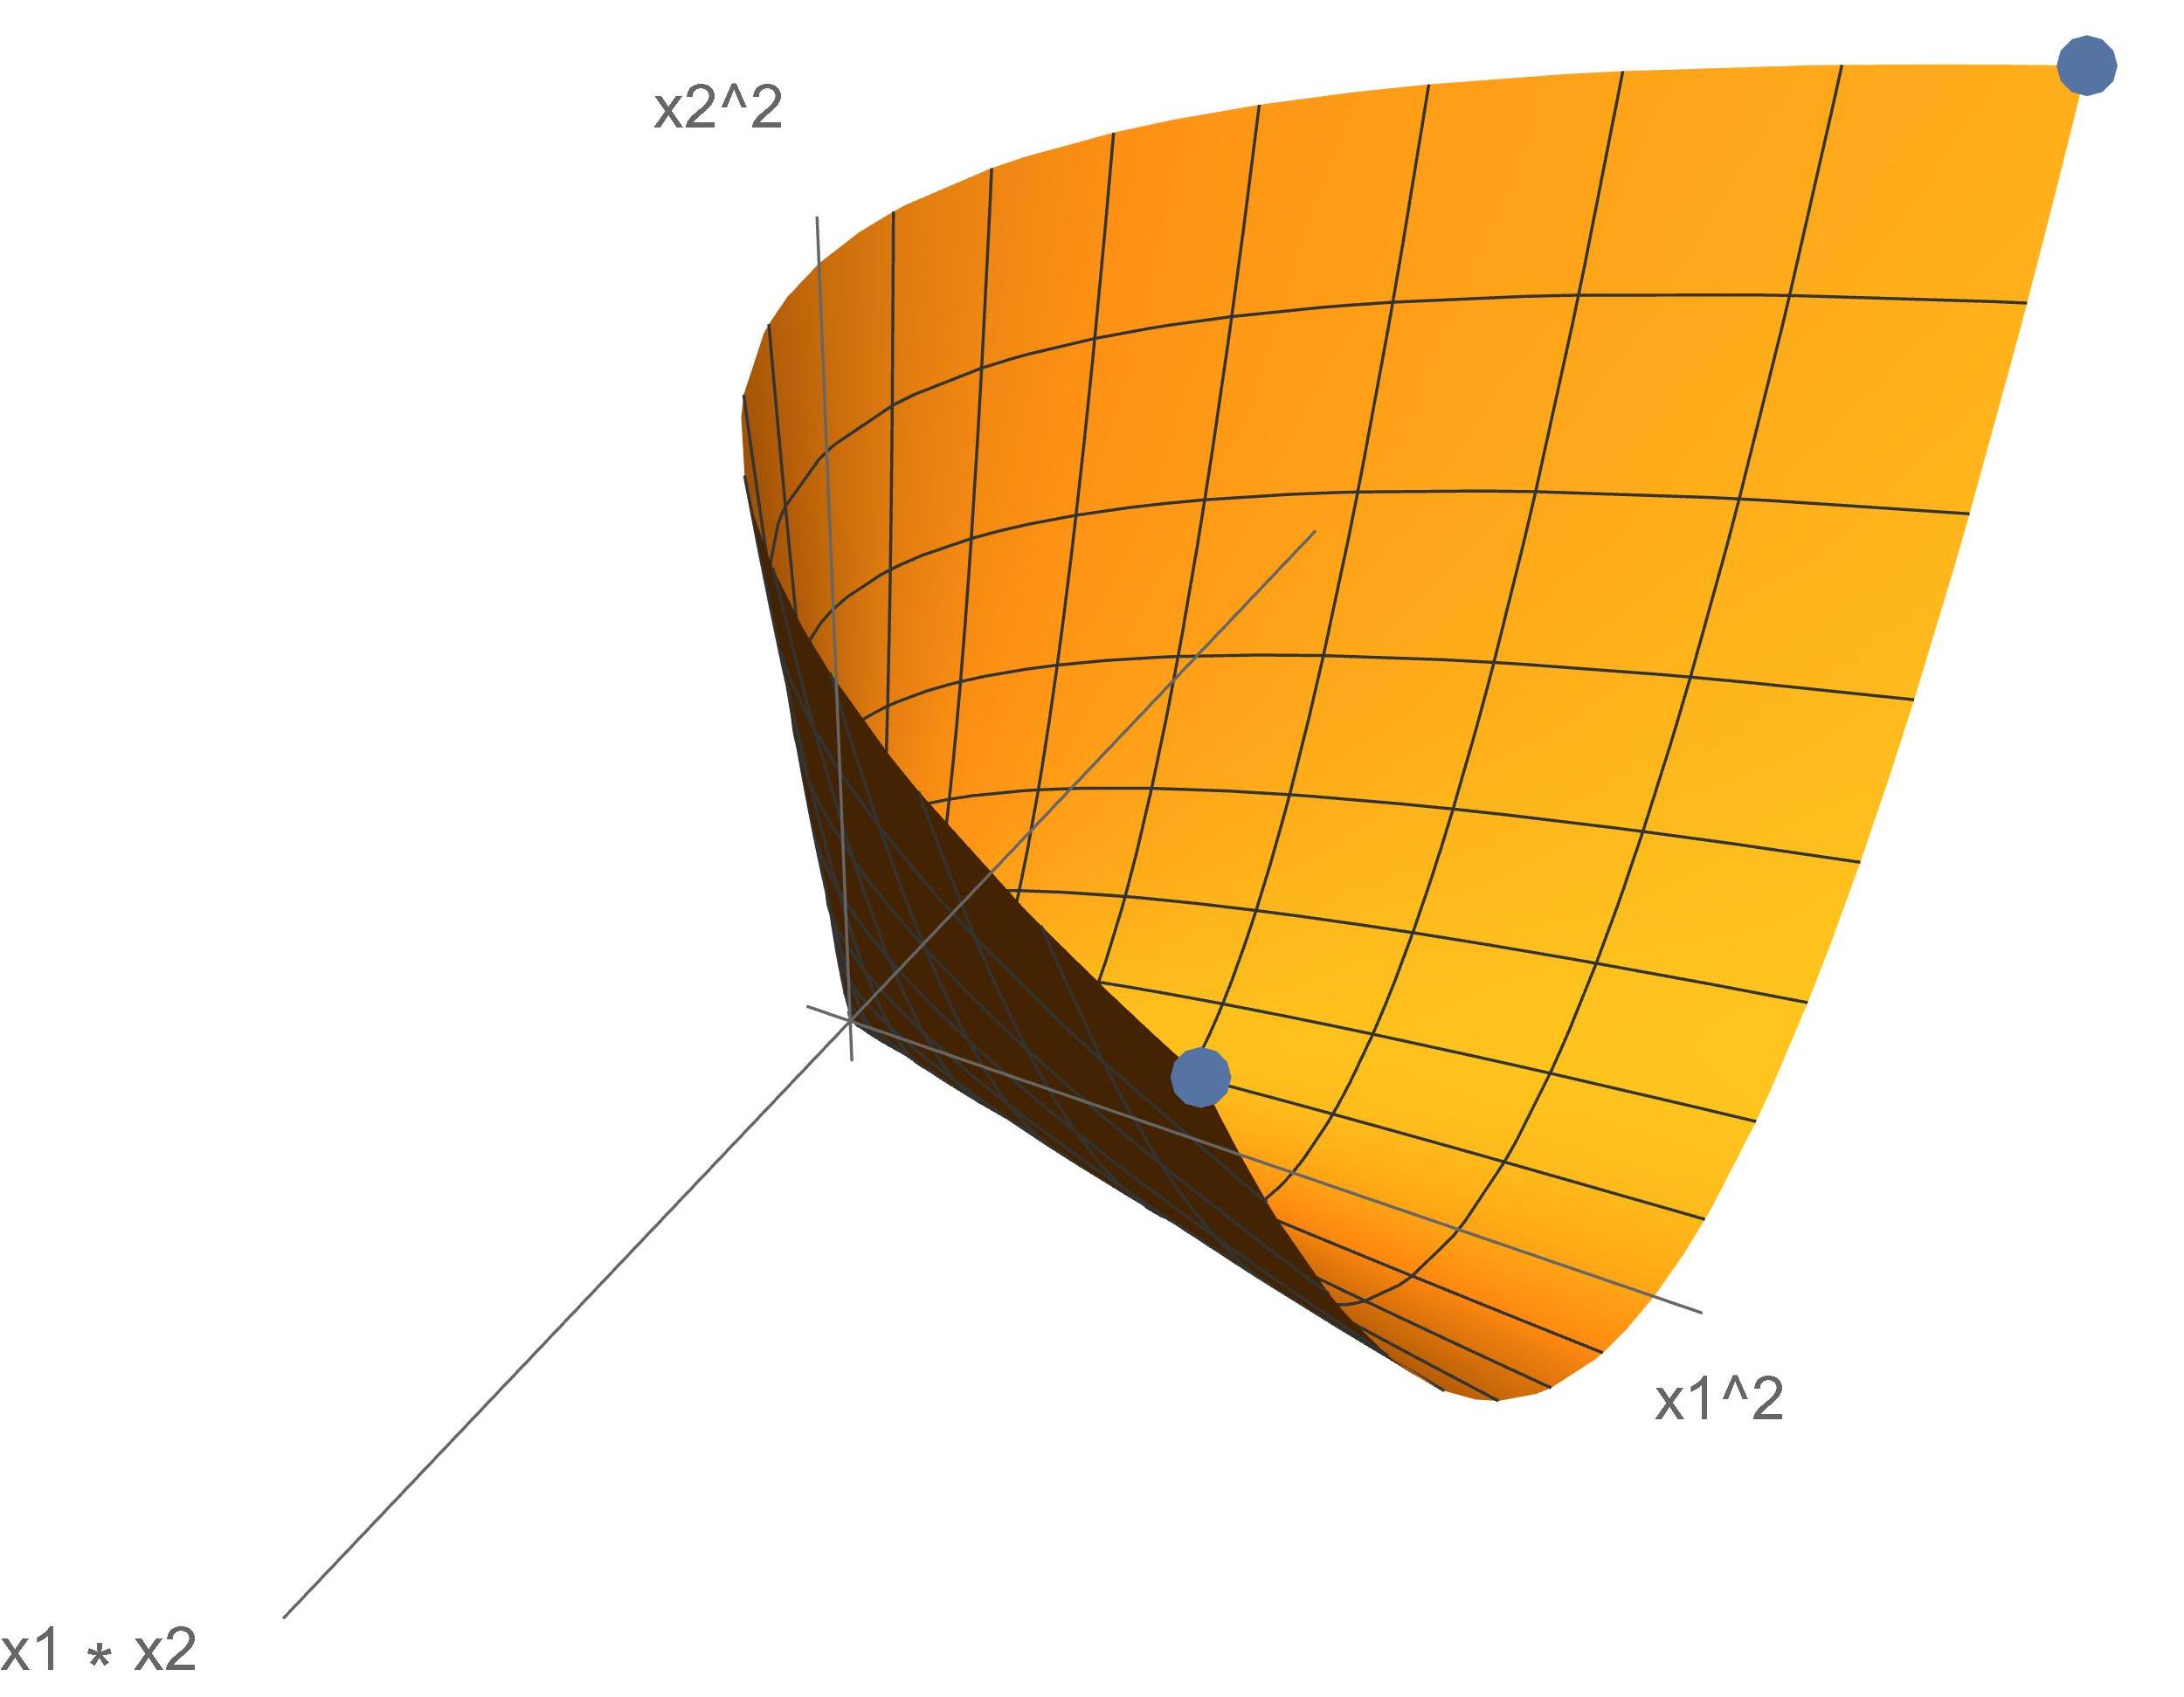
\includegraphics[width=\linewidth]{files/rank_one_matrices.jpg}
\end{figure}

Clearly, both homogeneity and the fact that we are working in $\R^2$ will play roles in any proof of Dines' Theorem.

\rule{0.5\linewidth}{\linethickness}

\begin{proof}
Let $Q(x)$, $Q(y)\in Q(\R^n)$ and for notational convenience, let
\begin{align*}
Q(x,y) \coloneqq \begin{pmatrix}
	x^\intercal A_1 y\\
	x^\intercal A_2 y
\end{pmatrix}.
\end{align*}

First, suppose $Q(x)$ and $Q(y)$ are collinear in $\R^2$. Then, as $Q(\R^n)$ is a \textit{cone}, i.e., $\alpha q \in Q(\R^n)$ for every $\alpha\geq 0$ and $q\in Q(\R^n)$, we have that the interval $[Q(x),Q(y)]$ is contained in $Q(\R^n)$.

Next, suppose $Q(x)$ and $Q(y)$ are not collinear.
Then, there exists a $v\in\R^2$ such that $\ip{v, Q(x)}, \ip{v,Q(y)} \geq \epsilon >0$ (i.e., $Q(x)$ and $Q(y)$ are both bounded away from the origin in some direction $v$). 

Now, let $z = (1- \mu) x + \mu (\pm y)$ where we will fix the sign $\pm$ later. In words, $z$ parameterizes the line containing $x$ and $\pm y$. Note that when $\mu = 0$ we have $Q(z) = Q(x)$, and when $\mu = 1$ we have $Q(z) = Q(\pm y) = Q(y)$.
We will pick the sign $\pm$ so that $Q(z)$ is also bounded away from the origin in the direction $v$ for all $\mu\in[0,1]$: Note that
\begin{align*}
\ip{v,Q(z)} &= \mu^2 \ip{v,Q(x)} + (1-\mu)^2 \ip{v,Q(y)}\\
&\qquad\pm 2\mu(1-\mu)\ip{v, Q(x,y)}.
\end{align*}
In particular, by picking the sign $\pm$ correctly, the last term above is nonnegative for all $\mu\in[0,1]$. Consequently, $\ip{v,Q(z)} \geq \epsilon/2>0$ for all $\mu\in[0,1]$. Finally, leveraging the geometry of $\R^2$ and the fact that $Q(\R^n)$ is a cone, we deduce that the interval $[Q(x), Q(y)]$ is contained in $Q(\R^n)$.
\end{proof}

\rule{0.5\linewidth}{\linethickness}
\section{What breaks for three quadratic forms?}
If we look over the above proof line by line to see what breaks when we go from two quadratic forms to three quadratic forms, we will see that not too much breaks.
Obviously, something does break because of the counterexample we saw earlier, but in fact the entirety of the proof remains intact save the very last sentence.

Specifically, in the case that $Q(x)$ and $Q(y)\in\R^3$ are not collinear, we can still find a continuous path between $Q(x)$ and $Q(y)$ contained in the image $Q(\R^n)$ and bounded away from zero in the direction $v$. Unfortunately, we may no longer conclude that the interval $[Q(x), Q(y)]$ is contained in $Q(\R^n)$, however, as this continuous path may \textit{loop}, so that it is not contained in the same plane as $Q(x)$ and $Q(y)$. See for example, the indicated points in the plotted figure above.

\rule{0.5\linewidth}{\linethickness}
\section{The power of $\C^n$}

Curiously, the three quadratic forms generalization of Dines' Theorem \textit{is true} when we switch from $\R^n$ to $\C^n$.

\begin{theorem}[{???\footnote{I remember reading about this result in some paper a while ago but don't remember the correct reference at the moment. Will fix later.}}]
Let $A_1,A_2,A_3\in\H^n$ be $n\by n$ Hermitian matrices. Then the image of $\C^n$ under the quadratic map $Q:\C^n\to\R^3$, given by
\begin{align*}
Q: x\mapsto \begin{pmatrix}
	x^* A_1 x\\
	x^* A_2 x\\
	x^* A_3 x
\end{pmatrix},
\end{align*}
is convex.
\end{theorem}

The main difference between $\R^n$ and $\C^n$, in this context, is that instead of simply being allowed to pick between a sign $\pm$ for $y$, we now have the freedom to pick $e^{i\theta}$ for any $\theta\in[0,2\pi)$. Or, perhaps more suggestively, we get to pick $\pm e^{i\eta}$ for both some sign and some $\eta\in [0,\pi)$.
This extra freedom, the choice of $\eta$, will allow us to force the continuous path that we construct between $Q(x)$ and $Q(y)$ onto the plane containing $Q(x)$ and $Q(y)$.
The rest of the proof follows analogously to Dines' Theorem.

{
\bibliographystyle{plainnat} 
\bibliography{bib.bib}
}


\end{document}